% Design document for the loading update of PoliVerse. Build: scripts/docs.sh
\documentclass[dd]{se2doc}
% Written once per project; every document reads it.
% Each document sets its own \docversion and \revision lines after reading this.
\project{PoliVerse Loading Update}
\authors{Samuele Segrini}
\docdate{10 November 2026}

\docversion{0.7}
\revision{0.1}{10 Nov 2026}{First draft, from RASD 1.0}
\revision{0.2}{10 Nov 2026}{After building M2: one stored value per key with the fetch time of each part (decision 2); Progress named LoadProgress; the loader's \texttt{updates} and \texttt{dueParts}}
\revision{0.3}{10 Nov 2026}{After building M3: the section kit as built (SectionStage, \texttt{arriving} with \texttt{hasRows}, \texttt{reveals}); the reveal's timing and when it plays}
\revision{0.4}{11 Nov 2026}{After building M4: RelevanceOrder, StableOrder and BoundaryClock as built; at a boundary only the rooms that change are asked about}
\revision{0.5}{11 Nov 2026}{After building M5: the deadline is applied by Query, which marks a part \texttt{late}; HostBreaker and HostPauses as built; only reads are answered from stored copies while a host is paused}
\revision{0.6}{11 Nov 2026}{After building M6: a resource says what a part changed, through ChangeDetector; NewMarks and the mark as built; LectureMoves for the timetable; the exam detector stays beside the generic one (decision 6)}
\revision{0.7}{11 Nov 2026}{After building M7: the budget is applied in RequestGate to every speculative request; LecturePrefetch runs TimetablePrefetch; floor plans through a loader; the settings in Dati e archiviazione; no 3D model to fetch}
% Domain terms, shared by every document.
\term{Screen}{One page of the app the student opens, such as Carriera or Aule libere.}
\term{Section}{A titled block of a screen that can be read on its own, such as the libretto inside Carriera.}
\term{Part}{The data behind one section: the answer to one request, or to one group of requests that only make sense together.}
\term{Stored copy}{A part kept on the phone from an earlier load, with the time it was fetched.}
\term{Max age}{How long a stored copy of a given kind of part is shown without asking the server again.}
\term{First content}{The first section of a screen that shows real data after the student opens it.}
\term{Speculative request}{A request the student did not ask for by opening a screen: a prefetch or an offline pack request.}
\term{Prefetch}{Fetching a part before the student opens the screen that shows it.}
\term{Offline pack}{The set of parts fetched ahead so that the app works with no connection.}
\term{Reveal}{The short animation with which arriving content writes itself onto the screen.}
\term{Loading ledger}{The on-device record of how long each part took and whether a speculative request was used.}
\term{Booking boundary}{A moment at which a room's booking starts or ends, so that the room changes between free and occupied.}
\term{Host}{One server of the Politecnico the app talks to, such as \texttt{api.polimi.it}.}
\term{Baseline}{The measurement taken with the loading ledger on the build before a change.}

\usepackage{float}
\usetikzlibrary{positioning,arrows.meta,fit}
% Requirement ids live in the RASD, so here they print as plain text.
\renewcommand\idref[1]{#1}
\lstset{language=Swift,numbers=none,xleftmargin=0pt,framexleftmargin=0pt}

% Sequence diagrams: \lifeline{name}{x}{label}, \msg[style]{from x}{to x}{y}{label}
\newcommand\seqdepth{8}
\newcommand\lifeline[3]{%
  \node[draw, font=\small, minimum height=0.6cm, inner xsep=5pt] (#1) at (#2,0) {#3};
  \draw[dashed, thin] (#1.south) -- (#2,-\seqdepth);}
\newcommand\msg[5][]{%
  \draw[-{Stealth[length=5pt]}, thin, #1] (#2,-#4) -- node[above=1pt, font=\scriptsize, inner sep=1pt, fill=white]{#5} (#3,-#4);}
\newcommand\selfmsg[3]{% x, y, label
  \draw[-{Stealth[length=5pt]}, thin] (#1,-#2) -- ++(0.5,0) -- ++(0,-0.35) -- ++(-0.5,0);
  \node[font=\scriptsize, anchor=west] at (#1+0.55,-#2-0.17) {#3};}

\traces{R1}{LoadProgress, Loader, Query, Section kit}
\traces{R2}{Query (LoadPhase), Section kit}
\traces{R3}{Query (\texttt{has}), Section kit}
\traces{R4}{LoadProgress (newest-only buffer), Loader (\texttt{updates}), Query}
\traces{R5}{Section kit (\texttt{arriving}, SectionStatus)}
\traces{R6}{Query (\texttt{failed}), Section kit (SectionStatus)}
\traces{R7}{Section kit (RevealRenderer), Query (\texttt{origin})}
\traces{R8}{Section kit (RevealRenderer)}
\traces{R9}{Section kit (\texttt{arriving} for lists)}
\traces{R10}{Section kit (\texttt{arriving})}
\traces{R11}{Section kit (ShapeMemory)}
\traces{R12}{Resource conformances, SearchModel}
\traces{R13}{RelevanceOrder, FreeRoomsModel}
\traces{R14}{Loader, OfflineStore}
\traces{R15}{Resource (\texttt{maxAge}), Loader}
\traces{R16}{Loader, OfflineStore}
\traces{R17}{DeadlinePolicy, Query (\texttt{late}), Section kit (LateLabel)}
\traces{R18}{HostBreaker, RequestGate, HostPauses, DataStatus}
\traces{R19}{TimetablePrefetch, LecturePrefetch, BackgroundRefresh, FreshnessCoordinator}
\traces{R20}{Loader (\texttt{warm}), FloorPlanResource, CoursePage}
\traces{R21}{OfflinePack, BackgroundRefresh}
\traces{R22}{OfflinePack, Impostazioni}
\traces{R23}{Loader, Query, Section kit}
\traces{R24}{BoundaryClock, FreeRoomsModel}
\traces{R25}{BoundaryClock, FreeRoomsModel, CampusMapModel}
\traces{R26}{ChangeDetector, Resource (\texttt{changes}), Loader}
\traces{R27}{NewMarks, Section kit (\texttt{newMark}, \texttt{clearsNewMarks})}
\traces{R28}{Query (\texttt{changes}, \texttt{onChanges}), NewMarks, Section kit (\texttt{newMark})}
\traces{R29}{LectureMoves, ChangeDetector, UpdateFeed, NotificationModel}
\traces{R30}{SpeculativeBudget, NetworkPath, RequestGate}
\traces{R31}{SpeculativeBudget, RequestGate}
\traces{R32}{RequestGate (lanes)}
\traces{R33}{SpeculativeBudget, SpeculativeCount, RequestGate, LecturePrefetch}
\traces{R34}{LoadingLedger, RequestGate}
\traces{R35}{LoadingLedger, Section kit (\texttt{screenLedger})}
\traces{R36}{LoadingLedger, Loader}
\traces{R37}{LedgerReport, DiagnosticsReport}
\traces{R38}{LoadingLedger (entry type)}
\traces{R39}{LoadingLedger, ReportArchive}
\traces{R40}{Loader (\texttt{clear}), OfflineStore, NewMarks, LoadingLedger}
\traces{P1}{Query, Section kit}
\traces{P2}{LoadProgress, Loader}
\traces{P3}{RelevanceOrder, FreeRoomsModel}
\traces{P4}{RequestGate, Loader}
\traces{P5}{OfflineStore, Loader (\texttt{restore})}
\traces{P6}{Section kit (RevealRenderer), LoadProgress}
\traces{P7}{TimetablePrefetch, Loader, LoadingLedger}
\traces{P8}{LoadingLedger}
\traces{P9}{OfflinePack, OfflineStore}

\begin{document}
\maketitle

% DRAFT, rewrite
\section{Introduction}

\subsection{Scope}
This document describes how the loading update specified in the RASD is built into
PoliVerse. It covers the changes to the store layer, the new components beside it,
the shared pieces of interface for a section's states, and the order in which they
are implemented and tested. It does not redesign the screens or the existing
networking code, and it adds no server.

\subsection{Definitions, acronyms, abbreviations}
The terms of the RASD apply. In addition:
\printterms

\noindent Store layer: the types under \texttt{PoliVerse/Model/Store}
(\texttt{Resource}, \texttt{Loader}, \texttt{Query}, \texttt{Env}, \texttt{HTTP}).
Lane: one of the two classes of request, on-screen or speculative.

\subsection{Reference documents}
Listed in section 7.

\subsection{Overview}
Section 2 gives the architecture: components, deployment, interfaces, runtime views
and the decisions taken. Section 3 describes the interface of a section. Section 4
traces requirements to components. Section 5 is the implementation, integration and
test plan.

% DRAFT, rewrite
\section{Architectural design}

\subsection{Overview}
The app keeps its four layers: views, observable models, the store layer and the
platform. The update adds no layer. It extends the store layer so that a load is
made of parts, and it adds a row of policies: small value types with no state of
their own that decide order, deadlines, budget, prefetch and changes. Policies take
the clock and the device state as arguments, so each is tested without a network,
a phone or waiting.

\begin{figure}[H]
\centering
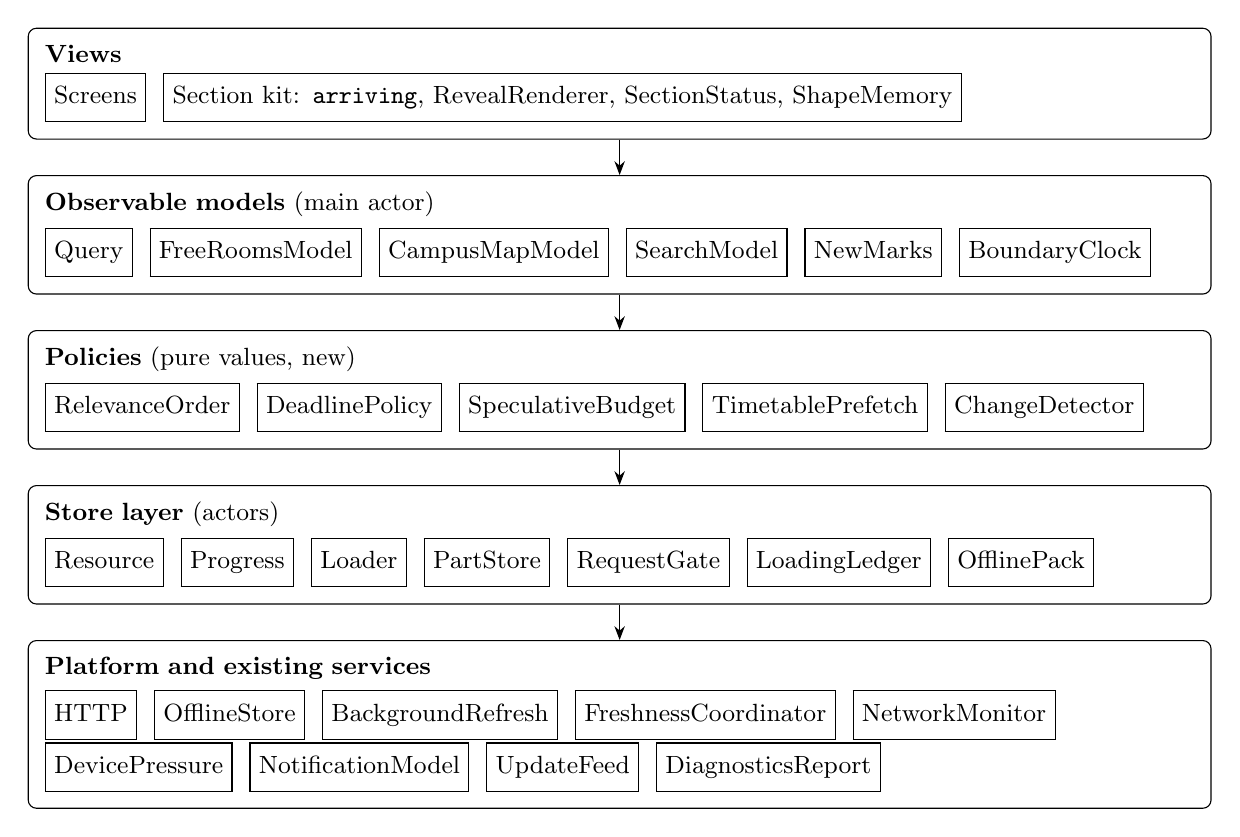
\begin{tikzpicture}[
  band/.style={draw, rounded corners=3pt, text width=14.6cm, align=left, inner sep=6pt, font=\small},
  uses/.style={-{Stealth[length=5pt]}, thin}]
  \newcommand\comp[1]{\fbox{\strut #1}\hspace{3pt}}
  \node[band] (ui) {\textbf{Views}\\[3pt]
    \comp{Screens} \comp{Section kit: \texttt{arriving}, RevealRenderer, SectionStatus, ShapeMemory}};
  \node[band, below=0.45cm of ui] (models) {\textbf{Observable models} (main actor)\\[3pt]
    \comp{Query} \comp{FreeRoomsModel} \comp{CampusMapModel} \comp{SearchModel} \comp{NewMarks} \comp{BoundaryClock}};
  \node[band, below=0.45cm of models] (policies) {\textbf{Policies} (pure values, new)\\[3pt]
    \comp{RelevanceOrder} \comp{DeadlinePolicy} \comp{SpeculativeBudget} \comp{TimetablePrefetch} \comp{ChangeDetector}};
  \node[band, below=0.45cm of policies] (store) {\textbf{Store layer} (actors)\\[3pt]
    \comp{Resource} \comp{Progress} \comp{Loader} \comp{PartStore} \comp{RequestGate} \comp{LoadingLedger} \comp{OfflinePack}};
  \node[band, below=0.45cm of store] (platform) {\textbf{Platform and existing services}\\[3pt]
    \comp{HTTP} \comp{OfflineStore} \comp{BackgroundRefresh} \comp{FreshnessCoordinator} \comp{NetworkMonitor} \comp{DevicePressure} \comp{NotificationModel} \comp{UpdateFeed} \comp{DiagnosticsReport}};
  \draw[uses] (ui) -- (models);
  \draw[uses] (models) -- (policies);
  \draw[uses] (policies) -- (store);
  \draw[uses] (store) -- (platform);
\end{tikzpicture}
\caption{Components by layer. An arrow means ``uses''; a layer also uses every layer below it.}
\end{figure}

\subsection{Component view}
New components are marked (new); the others exist and change.

\begin{description}[style=nextline, leftmargin=1.5em]
  \item[Resource] Declares one kind of remote data. Gains an optional \texttt{Part} type and a max age per part. A resource with one request declares nothing and compiles unchanged.
  \item[Progress (new)] The typed handle a fetch reports parts through. Replaces the untyped task-local \texttt{Partial.sink}. Holds only the newest snapshot not yet consumed.
  \item[Loader] One actor per resource. Now keeps an entry per part, asks the resource only for the parts that are missing or too old, files each part when it arrives, and applies the DeadlinePolicy.
  \item[PartStore (new)] Reads and writes one file per part and account on top of \texttt{OfflineStore}, with the fetch time. Written atomically.
  \item[Query] The observable handle a view reads. Gains which parts have arrived, which failed, where each came from (stored copy or network), and the changes of the last refresh.
  \item[RequestGate (new)] One actor for all hosts. Admits requests in two lanes, on-screen and speculative, caps speculative requests per host, tracks timeouts per host and fails fast while a host is not responding. Reports every request to the ledger.
  \item[LoadingLedger (new)] An actor that appends one small entry per request and per screen opening to a capped file, and computes the report.
  \item[RelevanceOrder (new)] Orders the rooms of a campus from the map area on screen, the next lecture's building and the favourite campus.
  \item[DeadlinePolicy (new)] Says, for a part and the time it has been waiting, whether to keep waiting or to show the stored copy.
  \item[SpeculativeBudget (new)] Says whether a speculative request may be sent now, from the network path, the device pressure, the student's settings and today's count.
  \item[TimetablePrefetch (new)] From the timetable and the current time, lists the parts to warm.
  \item[OfflinePack (new)] Owns the list of parts of the pack, runs it in a processing task, and publishes what is stored and how old.
  \item[BoundaryClock (new)] Computes the next booking boundary from stored bookings and wakes the models that show rooms.
  \item[ChangeDetector (new)] Compares the items of a fetched part with its stored copy by identity and returns what was added, changed and removed.
  \item[NewMarks (new)] Keeps, per account, the identities of items marked as new until their section has been on screen.
  \item[Section kit (new)] The shared interface pieces: the \texttt{arriving} modifier, RevealRenderer, SectionStatus and ShapeMemory.
  \item[Existing services] \texttt{BackgroundRefresh} gains the prefetch call and a processing task. \texttt{FreshnessCoordinator} calls the prefetch after a pass. \texttt{UpdateFeed} becomes one consumer of ChangeDetector. \texttt{DiagnosticsReport} gains the ledger section.
\end{description}

\subsection{Deployment view}
Everything runs on the student's iPhone. There is no server of the project.

\begin{center}\small
\begin{tabularx}{\linewidth}{@{}l X@{}}
  \toprule
  Node & What runs or lives there \\
  \midrule
  App process, foreground & All components. Requests run in both lanes. \\
  App process, refresh task & Agenda and career refresh as today, then TimetablePrefetch, within 30 seconds. \\
  App process, processing task & OfflinePack only. May be stopped by iOS at any time; resumes from PartStore. \\
  Widget extension & Reads the shared container, as today. Sends no request. \\
  App group container & PartStore files, NewMarks, the offline pack's state, the ledger file. \\
  Keychain & Tokens, as today. Never read by the new components. \\
  Politecnico's hosts & Answer HTTPS requests. Unchanged. \\
  \bottomrule
\end{tabularx}
\end{center}

\subsection{Component interfaces}
The signatures fix names and responsibilities; bodies and access levels are decided
in the code.

\begin{lstlisting}
// Resource: parts are optional. Part == Whole means "one request".
protocol Resource: Sendable {
    associatedtype Part: Hashable & Sendable & CaseIterable = Whole
    static func maxAge(of part: Part) -> TimeInterval        // default: ttl
    func fetch(_ key: Key, env: Env, parts: Set<Part>,
               over held: Value?, progress: Progress<Self>) async throws -> Value
}

struct Progress<R: Resource>: Sendable {
    func report(_ value: R.Value, arrived: Set<R.Part>, failed: Set<R.Part> = [])
}

actor Loader<R: Resource> {
    func value(_ key: R.Key, env: Env, force: Bool,
               progress: Progress<R>?) async throws -> Snapshot
    func warm(_ keys: some Sequence<R.Key>, env: Env)        // speculative lane
    func clear()                                             // sign-out
}

struct PartStore: Sendable {
    func save<V: Codable>(_ value: V, part: String, of name: String, account: String)
    func load<V: Codable>(_ type: V.Type, part: String, of name: String,
                          account: String) async -> (value: V, age: TimeInterval)?
    func removeAll(account: String)
}

@MainActor @Observable final class Query<R: Resource> {
    var value: R.Value? { get }
    func phase(of part: R.Part) -> LoadPhase
    func has(_ parts: R.Part...) -> Bool
    var changes: ChangeSet { get }                            // last refresh
}

enum LoadPhase: Equatable {
    case held(age: TimeInterval), waiting(since: Duration), arrived, empty
    case failed(String)
}

actor RequestGate {
    enum Lane { case onScreen, speculative }
    func run<T: Sendable>(host: String, lane: Lane, part: String,
                          _ request: @Sendable () async throws -> T) async throws -> T
    func isOpen(_ host: String) -> Bool                       // false while failing fast
}

actor LoadingLedger {
    func record(_ entry: RequestEntry)
    func opened(_ screen: String) -> ScreenToken
    func firstContent(_ token: ScreenToken)
    func completed(_ token: ScreenToken)
    func used(_ speculative: RequestID)
    func report(days: Int) async -> LedgerReport
    func erase()
}
\end{lstlisting}

\begin{lstlisting}
// Policies: values in, decision out. No clock, no singletons.
enum RelevanceOrder {
    static func order(_ rooms: [Classroom], visible: Set<BuildingID>,
                      nextLecture: BuildingID?, favourite: CampusID?) -> [Classroom]
}
struct DeadlinePolicy {
    var deadline: Duration = .seconds(4)
    func decision(waited: Duration, hasStoredCopy: Bool) -> Decision  // .wait | .showStored
}
struct SpeculativeBudget {
    struct Device { var lowData, metered, lowPower: Bool; var thermal: ThermalLevel }
    struct Settings { var allowMetered: Bool; var dailyLimit: Int = 600 }
    func allows(_ count: Int, device: Device, settings: Settings, sentToday: Int) -> Int
}
enum TimetablePrefetch {
    static func wanted(now: Date, lectures: [AgendaEvent],
                       lead: TimeInterval = 3600) -> [PrefetchItem]
}
enum ChangeDetector {
    static func changes<I: Identifiable & Equatable>(from old: [I], to new: [I]) -> ChangeSet
}
\end{lstlisting}

\begin{lstlisting}
// Section kit.
extension View {
    func arriving(_ phase: LoadPhase, title: LocalizedStringKey,
                  retry: (() async -> Void)? = nil) -> some View
    func revealed(order: Int, isNew: Bool) -> some View
    func screenLedger(_ name: String) -> some View
}
\end{lstlisting}

\subsection{Runtime view}

\subsubsection{UC1: a screen built from several parts}
\begin{figure}[H]
\centering
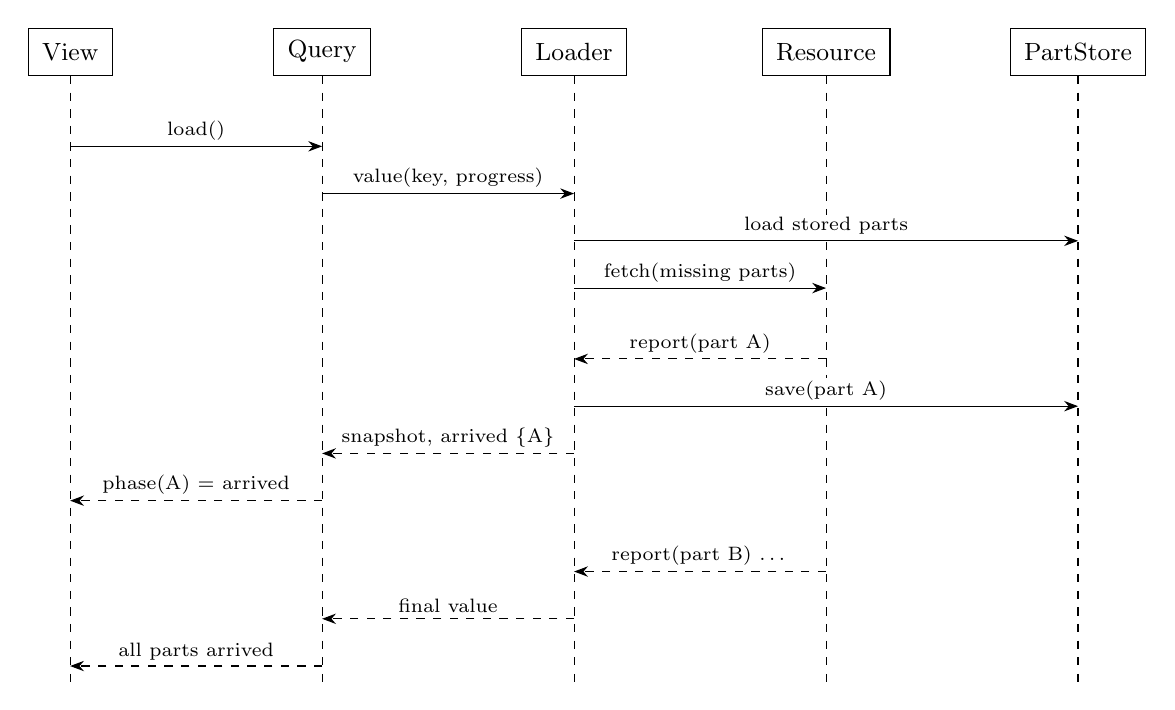
\begin{tikzpicture}
  \lifeline{v}{0}{View}
  \lifeline{q}{3.2}{Query}
  \lifeline{l}{6.4}{Loader}
  \lifeline{r}{9.6}{Resource}
  \lifeline{s}{12.8}{PartStore}
  \msg{0}{3.2}{1.2}{load()}
  \msg{3.2}{6.4}{1.8}{value(key, progress)}
  \msg{6.4}{12.8}{2.4}{load stored parts}
  \msg{6.4}{9.6}{3.0}{fetch(missing parts)}
  \msg[dashed]{9.6}{6.4}{3.9}{report(part A)}
  \msg{6.4}{12.8}{4.5}{save(part A)}
  \msg[dashed]{6.4}{3.2}{5.1}{snapshot, arrived \{A\}}
  \msg[dashed]{3.2}{0}{5.7}{phase(A) = arrived}
  \msg[dashed]{9.6}{6.4}{6.6}{report(part B) \dots}
  \msg[dashed]{6.4}{3.2}{7.2}{final value}
  \msg[dashed]{3.2}{0}{7.8}{all parts arrived}
\end{tikzpicture}
\caption{A load with parts. Each request inside \texttt{fetch} passes through RequestGate, which records it in the ledger.}
\end{figure}

The loader passes the resource only the parts that have no stored copy younger
than their max age (\idref{R15}, \idref{R16}). Reports are buffered newest-only and
the query consumes them at most every 100 ms (\idref{R4}). If the view goes away,
the fetch is cancelled as today, and the parts already saved stay (\idref{R14}).
When a part has waited longer than the deadline and a stored copy exists, the
loader hands the query that copy with \texttt{held(age:)} and keeps the request
running (\idref{R17}).

\subsubsection{UC2: free rooms}
\begin{enumerate}
  \item FreeRoomsModel asks RelevanceOrder for the order of the campus's rooms, giving it the buildings on the map, the next lecture's building and the favourite campus.
  \item It requests bookings eight at a time in that order through the occupancy loader, on the on-screen lane.
  \item After each batch it assigns the rooms received so far; the list and the map observe them.
  \item BoundaryClock computes the earliest booking boundary among the stored bookings and sleeps until then.
  \item At the boundary the model recomputes ``free now'' from stored bookings, and requests again the rooms on screen, once (\idref{R24}, \idref{R25}).
\end{enumerate}

\subsubsection{UC3: prefetch before a lecture}
\begin{figure}[H]
\centering
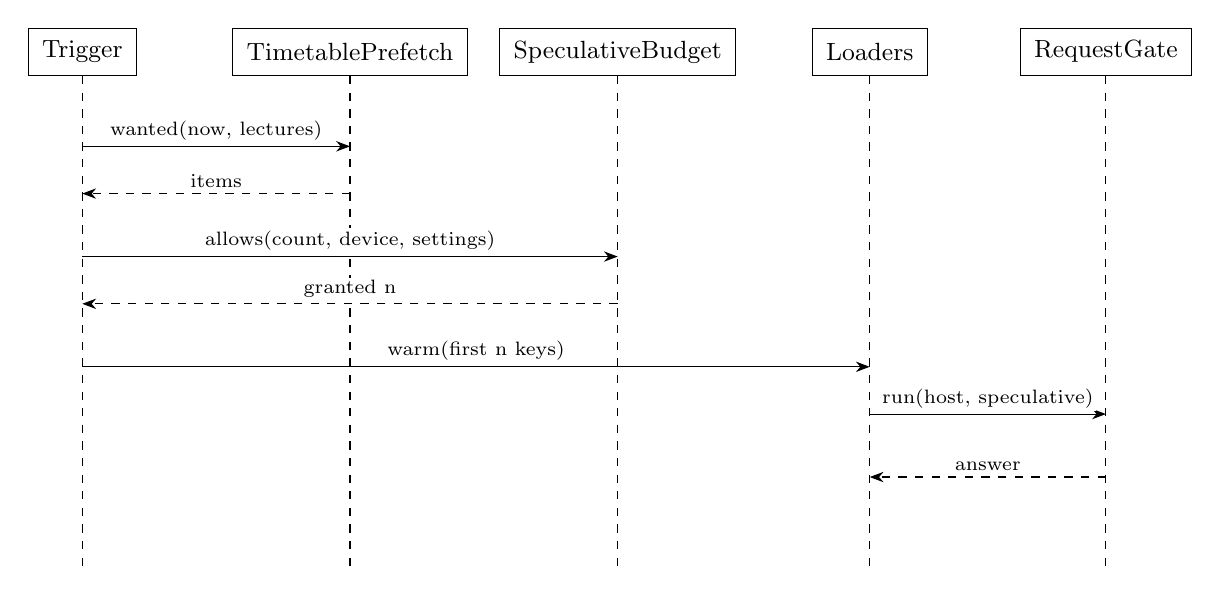
\begin{tikzpicture}
  \renewcommand\seqdepth{6.6}
  \lifeline{t}{0}{Trigger}
  \lifeline{p}{3.4}{TimetablePrefetch}
  \lifeline{b}{6.8}{SpeculativeBudget}
  \lifeline{l}{10.0}{Loaders}
  \lifeline{g}{13.0}{RequestGate}
  \msg{0}{3.4}{1.2}{wanted(now, lectures)}
  \msg[dashed]{3.4}{0}{1.8}{items}
  \msg{0}{6.8}{2.6}{allows(count, device, settings)}
  \msg[dashed]{6.8}{0}{3.2}{granted n}
  \msg{0}{10.0}{4.0}{warm(first n keys)}
  \msg{10.0}{13.0}{4.6}{run(host, speculative)}
  \msg[dashed]{13.0}{10.0}{5.4}{answer}
\end{tikzpicture}
\caption{Prefetch. RequestGate records each request in the ledger. The trigger is FreshnessCoordinator after a foreground pass, or BackgroundRefresh.}
\end{figure}

When the student later opens the room or the course, the loader finds the part
fresh and sends nothing (\idref{R20}); the ledger marks the speculative request as
used (\idref{R36}).

\subsubsection{UC4: no connection}
\begin{enumerate}
  \item The query asks the loader; the loader restores every stored part from PartStore.
  \item NetworkMonitor reports no connection, so RequestGate fails requests at once.
  \item Parts with a stored copy are \texttt{held(age:)}; parts without are \texttt{failed}; the section kit shows each accordingly (\idref{R23}).
  \item When the connection returns, FreshnessCoordinator runs a pass and only parts older than their max age are requested.
\end{enumerate}

\subsubsection{UC5: a change}
\begin{enumerate}
  \item A refresh brings a part that has a stored copy.
  \item Before filing it, the loader hands old and new items to ChangeDetector.
  \item The change set goes to the query (\texttt{changes}), to NewMarks, and to UpdateFeed, whose existing policy decides whether to notify (\idref{R29}).
  \item The section kit reveals only items in the change set and shows the mark; when the section has been on screen, NewMarks removes them (\idref{R27}, \idref{R28}).
\end{enumerate}

\subsubsection{UC6: the ledger}
\texttt{screenLedger} opens a token when a screen appears, the first \texttt{arriving}
section to reach \texttt{arrived} or \texttt{held} marks first content, and the
last marks completion. DiagnosticsReport asks the ledger for the report over 14
days.

\subsection{Selected architectural styles and patterns}
\begin{itemize}
  \item \textbf{Layers}, as today: a view never talks to a loader, a loader never to a view.
  \item \textbf{Functional core, imperative shell}: decisions live in policies that are pure; actors and models only carry them out.
  \item \textbf{Actors for coordination}: Loader, RequestGate and LoadingLedger hold shared state; work proportional to a payload stays in \texttt{@concurrent} functions.
  \item \textbf{Observer} through Observation: models are \texttt{@Observable} on the main actor.
  \item \textbf{Stale-while-revalidate}, now per part.
  \item \textbf{Circuit breaker} per host, inside RequestGate.
\end{itemize}

\subsection{Other design decisions}
\begin{description}[style=nextline, leftmargin=1.5em]
  \item[1. Progress is a parameter, not a task-local.] Alternative: keep \texttt{Partial.sink}. A task-local cannot be generic, so it is untyped and cast back, and it cannot say which parts arrived. Cost: the \texttt{fetch} signature changes; a default implementation forwards to the old one for resources without parts.
  \item[2. One file per part.] Alternative: one file per resource, rewritten when each part arrives. Per-part files make each write small and atomic, so a kill between two parts loses nothing (\idref{R14}, \idref{R16}), and each carries its own age (\idref{R15}). Cost: restoring reads several small files; \idref{P5} bounds it.
  \item[3. A deadline shows the stored copy and keeps the request.] Alternatives: cancel and retry, or send a second request in parallel. Both add load on the Politecnico's hosts, against assumption D11, and a late answer is still the freshest data.
  \item[4. The breaker is per host, in one gate.] Alternative: per resource. A timeout says something about the host, and all resources on that host benefit at once (\idref{R18}). One gate is also the only place that sees every request, which the ledger and the lanes need.
  \item[5. Prefetch follows the timetable, not habits.] Relies on assumption D5. A learned predictor needs data the ledger does not have yet and is out of scope.
  \item[6. Changes are found by identity, generically.] Alternative: one detector per kind of data, as UpdateFeed does today for exams. Relies on assumption D10. Values expose their items as \texttt{Identifiable \& Equatable}; kinds without stable ids are not compared.
  \item[7. The ledger is the app's own file.] Alternatives: signposts or MetricKit alone. Signposts cannot be read back on the phone, and MetricKit delivers one aggregate a day without per-part detail. The ledger stores no content (\idref{R38}).
  \item[8. A boundary is one sleep until a known instant.] Relies on assumption D6. It is not polling: nothing is sent unless a boundary passed and the screen is visible.
  \item[9. The offline pack uses a processing task.] The refresh task's 30 seconds cannot hold it (assumption D7). The pack is resumable because every part is filed when it arrives.
  \item[10. No separate package yet.] The store layer stays in the app target until this update has shipped; \texttt{Packages/} is also ignored by git today. Moving it is a later, mechanical step.
\end{description}

% DRAFT, rewrite
\section{User interface design}

\subsection{A section's states}
Screens do not draw their own spinners or empty states for a part. A section's rows
are wrapped in \texttt{arriving(phase, hasRows:, title:)}, which draws exactly one of
these. Rows already on screen stay there whatever their part is doing: the status
replaces only rows that do not exist.

\begin{center}\small
\begin{tabularx}{\linewidth}{@{}l X X@{}}
  \toprule
  Phase & What is drawn & Accessibility \\
  \midrule
  \texttt{held} & The content. & Read as content. \\
  \texttt{late} & The content, under one line: ``Dati di 12 min fa, sto aggiornando''. The line goes when the answer arrives. & The line is read before the content. \\
  \texttt{waiting}, under 300 ms & The remembered height, empty. & Hidden. \\
  \texttt{waiting}, over 300 ms & The title and one soft waiting line where the first text line will be. & One element: ``Caricamento'' and the title. \\
  \texttt{waiting}, over 3 s & The same, plus the step in progress or ``120 di 340''. & The step is read once. \\
  \texttt{arrived} & The content, with the reveal if it is new. & Announced if the wait passed 3 s. \\
  \texttt{empty} & The section's empty-state message. & Read as content. \\
  \texttt{failed} & One line naming what is unavailable and ``Riprova''. & A button. \\
  \bottomrule
\end{tabularx}
\end{center}

A service that is paused after two timeouts is named once for the whole app, in
the status line: ``Carriera non risponde: mostro i dati salvati'', or the count
when there are several. Sections say nothing more than their \texttt{late} or
\texttt{failed} state.

\subsection{The reveal}
\begin{itemize}
  \item Text: a \texttt{TextRenderer} gives each group of five glyphs, about a word, opacity 0 to 1, blur 6 to 0 pt and a 2 pt rise, staggered so that the whole text ends within 0.6 s; only the first three lines animate piece by piece, the rest fade as one. The layout a renderer receives has glyphs and runs, not words.
  \item Rows and cards: opacity, a 6 pt blur and a 2 pt rise over 0.3 s, each starting 0.05 s after the one above and none later than 0.3 s, so the section ends within 0.6 s however long it is.
  \item Numbers: \texttt{.contentTransition(.numericText(value:))}.
  \item On a refresh over visible content, only the rows the refresh added or changed replay their reveal, and their mark comes in with it. Every other row stays as it is.
  \item The reveal plays only when rows arrive from the network in a section that was seen waiting. Rows that are there when the screen opens, a stored copy, or a day paged to are drawn at once.
  \item A tap or a scroll ends the reveal at once. Reduce Motion replaces it with a 0.2 s cross-fade and removes the waiting line's movement.
\end{itemize}

\subsection{New and changed items}
A row that a refresh added or changed carries a mark: a small dot in the accent
colour at its top trailing corner, read by VoiceOver as ``Nuovo'' after the row.
In the libretto a closed year carries the mark when one of its results does. The
marks of a section go away once the section has been on screen for at least a
second and the student leaves it or puts the app away; a section flicked past
keeps them. Appelli and Libretto in Carriera are the first sections with marks.

\subsection{Lists that grow}
A list that receives rows while the student has scrolled adds them below the
visible rows. A sorted list that would reorder waits for the scroll to stop, then
moves rows with the system's default list animation. Aule libere is the first such
list: while a campus is arriving the rooms shown keep their places, a line under
the header says how many rooms have answered, and ``nessuna aula libera'' is not
said until the whole campus has.

\subsection{Map and 3D}
Building colours on the map follow the order of arrival, which RelevanceOrder makes
the order of distance from what is on screen. A building's 3D shell fades in by
opacity when its model has loaded; no other effect is used, because shadows are
what costs frames on the iPhone 12 Pro.

\subsection{New pages in Impostazioni}
\begin{itemize}
  \item \textbf{Offline}: a switch for the pack, one row per item with ``pronto'' and its age or ``non ancora scaricato'', the space used, and ``Scarica ora''.
  \item \textbf{Dati e archiviazione}, which exists, gains a section ``Preparazione in anticipo'' rather than a page of its own: ``Prepara in anticipo'' on by default, ``Anche con la rete cellulare'' off by default and shown only while the first is on, and ``Richieste in anticipo oggi'' with today's count against the limit. The footer says what is prepared and when it is not.
  \item \textbf{Promemoria}, which exists: the switches for the kinds of news gain ``Lezioni spostate''; marks and sittings already had theirs. A new switch at the foot of the page, ``Vibrazione all'arrivo dei dati'', off by default, enables the haptic of \idref{R10}.
\end{itemize}

\subsection{Diagnostics}
The diagnostics report gains ``Caricamento'': per screen, the median and 90th
percentile of time to first content and to the last part; per kind of part, the
same for its duration and its share of failures; the share of speculative requests
used; and ``campione troppo piccolo'' under 20 openings.


\section{Requirements traceability}
Every requirement of the RASD maps to at least one component, and every component of
section 2.2 appears at least once.
\printtraceability

% DRAFT, rewrite
\section{Implementation, integration and test plan}

\subsection{Order of implementation}
Eight milestones, each shippable by itself on the existing branch. The ledger
comes first so that every later milestone is measured against a baseline. The two
changes to the store layer's interface come second, before any screen depends on
the old one.

\begin{center}\small
\begin{tabularx}{\linewidth}{@{}l X l@{}}
  \toprule
  Milestone & Content & Requirements \\
  \midrule
  M1 Ledger & RequestGate as a pass-through that records; LoadingLedger; the report; \texttt{screenLedger} on the main screens; baseline run on the iPhone 12 Pro & R34 to R39, P8 \\
  M2 Parts & \texttt{Part} and \texttt{maxAge} on Resource; LoadProgress; per-part Loader and stored part times; Query's phases; the career as first user; search in parallel & R1 to R3, R12, R14 to R16, R40 \\
  M3 Section kit & \texttt{arriving}, SectionStatus, RevealRenderer, ShapeMemory; applied to Carriera, Appelli, Libretto and Oggi & R4 to R11, P1, P2, P6 \\
  M4 Rooms & RelevanceOrder; free rooms assigned per batch; map colours; BoundaryClock & R13, R24, R25, P3 \\
  M5 Slow parts & DeadlinePolicy in the loader; the host breaker in RequestGate & R17, R18 \\
  M6 Changes & ChangeDetector; \texttt{changes} on Query; NewMarks; UpdateFeed as a consumer; the new notification kinds & R26 to R29 \\
  M7 Prefetch & SpeculativeBudget; lanes in RequestGate; TimetablePrefetch; its two triggers; the settings page & R19, R20, R30 to R33, P7 \\
  M8 Offline & OfflinePack and its processing task; the Offline page; behaviour with no connection on every screen of the pack & R21 to R23, P5, P9 \\
  \bottomrule
\end{tabularx}
\end{center}

P4, the time to the last part, is checked at the end of every milestone against the
baseline of M1.

\subsection{Integration strategy}
Bottom-up, following the layers. Within a milestone: first the policy, alone, with
its unit tests; then the actor or model that uses it, against a stub transport;
then the screens. A component is merged only when the layer under it is tested, so
no stubs of lower layers are needed except the transport and the clock.
RequestGate and LoadProgress are thread-like dependencies of everything after them,
which is why they are in M1 and M2.

\subsection{Test plan}
\begin{description}[style=nextline, leftmargin=1.5em]
  \item[Static analysis] The existing checks: \texttt{scripts/swiftcheck.py} and \texttt{scripts/check-model-layer.sh}, with Swift 6 strict concurrency as the compiler's own analysis.
  \item[Unit] Every policy (RelevanceOrder, DeadlinePolicy, SpeculativeBudget, TimetablePrefetch, ChangeDetector) and the ledger's statistics, with values and a fixed clock. Each test's name carries the requirement's id, for example \texttt{test\_R13\_visibleBuildingsFirst}.
  \item[Integration] Loader with OfflineStore and RequestGate over a stub resource or \texttt{HTTP} that answers parts in a scripted order, after scripted delays on a test clock, or never. This is where \idref{R1} to \idref{R3}, \idref{R14} to \idref{R18} and \idref{R40} are tested: arrival in any order, a kill between two parts, a part that never answers, sign-out.
  \item[System] UI tests on the simulator with fixtures: each state of a section is reached and asserted through its accessibility element; Reduce Motion; no connection. Then the device bench on the iPhone 12 Pro for \idref{P1} to \idref{P9}, read from the ledger.
  \item[Acceptance] UC1 to UC6 played by hand on the phone with a real account, including a real trip with no signal for UC4.
\end{description}

\subsection{What is hard to test, and how}
\begin{itemize}
  \item Background tasks cannot be forced on a phone outside the debugger. The prefetch and the pack are functions called by the task handlers, tested directly; the handlers themselves are exercised with the debugger's simulate commands.
  \item Notifications for changes need a change on the server. ChangeDetector and the policy are tested with fixtures; one acceptance run waits for a real change.
  \item The reveal's cost depends on the phone. \idref{P6} is measured on the iPhone 12 Pro only, in the same interleaved rounds used for the 3D bench.
\end{itemize}


\section{Effort spent}
% TODO: one \effort{task}{hours} per task, then \printeffort.
To be recorded as the work proceeds.

\section{References}
\begin{enumerate}
  \item \emph{PoliVerse Loading Update, RASD}, version 1.0.
  \item \texttt{docs/data-loading-architecture.md}: the store layer as built.
  \item \texttt{docs/data-freshness.md}: refresh triggers and what the servers return.
  \item \emph{Partial loading in PoliVerse} and \emph{New capabilities for partial loading}, analysis documents, 10 November 2026.
  \item Apple, \emph{Create custom visual effects with SwiftUI}, WWDC24, for \texttt{TextRenderer}.
  \item Apple, BackgroundTasks, Network and UserNotifications framework documentation.
\end{enumerate}

\end{document}
